\documentclass[../dissertation.tex]{subfiles}

\begin{document}
We have defined tangent-point energy quadrature for simple closed curve (any curve homeomorphic to circle) $\gammabf$ at (\ref{equ: Tangent-Point Energy Quadrature}).

For curves in different homeomorphism class from $S^1$,
one may make minor changes to (\ref{equ: Tangent-Point Energy Quadrature}) to get a sensible quadrature.

\subsection{Curves Homeomorphic to a Line Segment}
Given a curve $\gammabf$ homeomorphic to a line segment,
one could take the following as its tangent-point energy quadrature for its discretisation $\Gammabf^k$:
\begin{equation}
    E_{\beta}^{\alpha} \left( \Gammabf^k \right) \coloneqq \sum_{\substack{i,j \in \left\{ 1, \cdots, N-2 \right\} \\ r\left( i-j,N \right) > 1}} K_{\beta}^{\alpha} (i,j) \norm{e_i} \, \norm{e_j}
\end{equation}
where the contribution from each end is neglected.
Note that unlike a simple closed curve,
one does not generalise the indexing rule to be ``cyclic''.

\subsection{Curves Homeomorphic to Bus Network}
\begin{figure}[tpb]
    \centering
    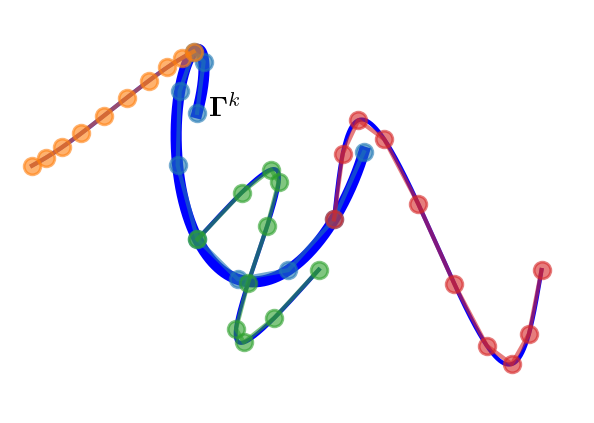
\includegraphics[]{sections/otherHomeomorphismImgs/branch}
    \caption{A curve with branches from a main ``stem''.}
    \label{fig: Bus Network}
\end{figure}
For a curve $\gammabf$ that has $m$ ``branches'', one needs to take into account of at what points on the discretisation branching happens.
Suppose for all branches protrude from a single ``stem''.
On Figure \ref{fig: Bus Network}, the stem is represented by the thick blue curve.

One can capture this curve by a tensor of the following form.
\begin{equation*}
    \Gammabf^k = \left( \underbrace{\xbf_{0,0}^k, \cdots, \xbf_{0,n_0}^k}_{\text{Stem}} \middle|
    \underbrace{\xbf_{1,0}^k, \cdots, \xbf_{1,n_1}^k}_{\text{Branch 1}}
\middle| \cdots \middle|
\underbrace{\xbf_{m,0}^k, \cdots, \xbf_{m,n_m}^k}_{\text{Branch } m}\right)
\end{equation*}
where the ``linkage points'' for branches to the stem are $\xbf_{1,0}^k, \cdots, \xbf_{m,0}^k$,
which can be identified by the fact that $\xbf_{1,0}^k, \cdots, \xbf_{m,0}^k \in \left\{ \xbf_{0,0}^k, \cdots, \xbf_{0, n_0}^k \right\}$,
that is, all duplicate points are to be understood as linkage points.
Denote the set of linkage points as $L \left( \Gammabf^k \right)$.
Note that this is a natural generalisation of discretisation of curves homeomorphic to a line segment.


\end{document}
